\documentclass[utf8]{beamer}\usepackage[]{graphicx}\usepackage[]{color} %,handout
%% maxwidth is the original width if it is less than linewidth
%% otherwise use linewidth (to make sure the graphics do not exceed the margin)
\makeatletter
\def\maxwidth{ %
  \ifdim\Gin@nat@width>\linewidth
    \linewidth
  \else
    \Gin@nat@width
  \fi
}
\makeatother

\usepackage{framed}
\makeatletter
\newenvironment{kframe}{%
 \def\at@end@of@kframe{}%
 \ifinner\ifhmode%
  \def\at@end@of@kframe{\end{minipage}}%
  \begin{minipage}{\columnwidth}%
 \fi\fi%
 \def\FrameCommand##1{\hskip\@totalleftmargin \hskip-\fboxsep
 \colorbox{shadecolor}{##1}\hskip-\fboxsep
     % There is no \\@totalrightmargin, so:
     \hskip-\linewidth \hskip-\@totalleftmargin \hskip\columnwidth}%
 \MakeFramed {\advance\hsize-\width
   \@totalleftmargin\z@ \linewidth\hsize
   \@setminipage}}%
 {\par\unskip\endMakeFramed%
 \at@end@of@kframe}
\makeatother

\usepackage{alltt}
\hypersetup{colorlinks}
\usetheme{Luebeck}
%\usecolortheme{spruce}
\useoutertheme{infolines}
\setbeamertemplate{bibliography item}{\insertbiblabel}
\useinnertheme{rectangles}
\usefonttheme{professionalfonts}
\setbeamercovered{%
still covered={\opaqueness<1->{15}},
again covered={\opaqueness<1->{40}}}

% using Lucida bright as in TUG distribution
%\usepackage[T1]{fontenc}
%\usepackage{textcomp}
%\usepackage[altbullet]{lucidabr}

\usepackage{tikz}
\usetikzlibrary{positioning,fit,arrows}

\tikzset{
 a/.style
  = {node distance=4em, text width=2.7em, minimum height=4em},
 b/.style
  = {rectangle, draw, fill=gray!10, node distance=4em, text width=6em,
     text centered, rounded corners, minimum height=4em, thick},
 c/.style
  = {circle, draw, dashed, fill=orange!10, inner sep = 0pt, node distance=5em, thick},
 d/.style
  = {rectangle, draw, dashed, fill=red!10, node distance=4em, text width=6em,
     text centered, rounded corners, minimum height=4em, thick},
 l/.style
  = {draw, -latex, thick},
 lr/.style
  = {draw, latex-latex, thick, red},
 lb/.style
  = {draw, -latex, thick, blue},
  lo/.style
  = {draw, -latex, thick, orange},
  lg/.style
  = {draw, -latex, thick, green},
  mylabel/.style
  ={text width=6.5em, text centered}
}

\usepackage[sortcites,autocite=superscript]{biblatex}
\addbibresource{research.bib}
\addbibresource{pja.bib}
%\renewcommand{\bibfont}{\footnotesize}

%\usepackage{abbrev}


% \bibpunct{(}{)}{,}{a}{}{,}
%
% \newcommand\hangbibentry[1]{%
%     \smallskip\par\hangpara{1em}{1}\bibentry{#1}\smallskip\par %{indent}{afterline}
% }

\title{Can plants predict the future?}
\subtitle{How and why?}
\author{Pedro J. Aphalo}
\date{\emph{Eco Evo Seminar}\\ 2016-03-31}
\pgfdeclareimage[height=1cm]{mylogo}{figures/senpep_logo}
\institute[SenPEP]{ViPS, Department of Biosciences, University of Helsinki\\[2ex] \pgfuseimage{mylogo}}

\IfFileExists{upquote.sty}{\usepackage{upquote}}{}

\begin{document}

\setbeamercovered{%
still covered={\opaqueness<1->{5}},
again covered={\opaqueness<1->{35}}}

\begin{frame}
\maketitle
\end{frame}

\begin{frame}[c]
\begin{center}
\begin{small}
\copyright 2014--2016 by Pedro J. Aphalo and others\\
Department of Biosciences, University of Helsinki, Finland.\\
\textcolor{blue}{\url{http://blogs.helsinki.fi/aphalo/}}\\[2ex]
\end{small}

\begin{footnotesize}
`Sensory Ecology: Is it applicable to plants?'
by Pedro J. Aphalo is licensed under a Creative Commons Attribution-ShareAlike 4.0 International License.\\[2ex]
\end{footnotesize}

\includegraphics[width=6em]{copyright/by-sa}
\end{center}
\end{frame}


\begin{frame}
\frametitle{Outline}
\tableofcontents
\end{frame}

\section{Background}

\begin{frame}[<+->]
  \frametitle{Physiology and molecular biology studies}
  \framesubtitle{Evolutionary viewpoint frequently missing}
  \begin{itemize}
    \item Looking at the sensory abilities of organisms from an evolutionary and fitness perspective should be nothing new for today's audience.
    \item In the case of plants this approach has been rarely used\ldots
    \item \ldots based on the assumption that sensory capabilities and specially information processing are very limited in plants.
    \item Now we know that this assumption does not hold.
  \end{itemize}
\end{frame}

\begin{frame}[<+->]
  \frametitle{Plants' ``senses''}
  \framesubtitle{What can plants perceive}
  \begin{itemize}
    \item Light amount (`moonlight' to full sun).
    \item Light wavelength (270~nm to $\approx$ 800 nm).
    \item Light direction.
    \item Temperature.
    \item Gravity.
    \item Mechanical stimulus.
    \item Chemoperception (volatiles in the atmosphere, solutes in the soil).
    \item Magnetic fields (?).
    \item Electric fields (?).
    \item Sounds and mechanical vibration (?).
  \end{itemize}
\end{frame}

\begin{frame}[<+->]
  \frametitle{Plant-plant ``communication''}
  \framesubtitle{Emission of informational signals}
  \begin{itemize}
    \item Volatiles to the atmosphere:
    \begin{itemize}
      \item These are sophisticated cocktails that carry information about the species of
      pathogen or herbivore attacking the emitter
      \item These signals are `used' by neighbouring plants, but also in the case of herbivores,
      attract the predators of the herbivores.
    \end{itemize}
    \item Chemicals to the soil as warning signals (?) and territorial marks (????).
    \item Information transfer from plant to plant with mycorrhizal fungi as middlemen (??).
    \item Light signals (reflection) to deceive neighbours (???), but also attract pollinators.
  \end{itemize}
\end{frame}

\begin{frame}[<+->]
  \frametitle{Within plant ``communication''}
  \framesubtitle{Coordination}
  \begin{itemize}
    \item Plants have a modular architecture.
    \begin{itemize}
      \item Each ``module'' is to some extent autonomous but exchanges information with the rest of the plant.
      \item The information moves fast in some cases (minutes).
    \end{itemize}
    \item Plant ``hormones'', small proteins, miRNA, VOCs and electric potentials (??) carry signals within the plant.
  \end{itemize}
\end{frame}

\begin{frame}[<+->]
  \frametitle{Plants' ``intelligence''}
  \framesubtitle{Information processing}
  \begin{itemize}
     \item Detection of timing of events (based on circadian clock).
    \item Detection of spatial and temporal gradients.
     \item Ability to combine information from several sources, leading to different outcomes.
     \begin{itemize}
       \item positive and negative interactions.
       \item responses dependent on ratios.
       \item responses dependent on temporal sequence of stimuli.
     \end{itemize}
    \item Plants store information for different lengths of time:
    \begin{itemize}
      \item from minutes to a lifetime within their lifetime.
      \item maternal effects such trans-generational epigenetic `memory'.
    \end{itemize}
  \end{itemize}
\end{frame}

\begin{frame}[<+->]
  \frametitle{Forecasting}
  \framesubtitle{Is it a useful concept in relation to fitness?}
  \begin{itemize}
    \item We depend on informally forecasting all sorts of events every minute while awake.
    \item Sometimes we do this consciously, but most of the time we are not aware of what our brain is doing.
    \item We use forecasts at very different time scales and to many different ends.
    \item If we use the abstraction of information, and for a moment forget about how its processing is implemented\ldots
    \item \ldots it is easy to imagine that every organism must have evolved the capacity to ``forecast'' future events important for fitness.
    \item How information is processed, ``the machinery used'', does not need to be the same as long the information is acquired, transmitted, stored and combined succesfully.
  \end{itemize}
\end{frame}

\begin{frame}[<+->]
  \frametitle{Can plants forecast the future?}
  \framesubtitle{Preemptive acclimation}
  \begin{itemize}
    \item Several plant responses can be only explained from the evolutive/fitness
    point of view as being a `preparation' to tolerate or escape future stress events or
    take advantage of future favourable conditions.
    \begin{itemize}
    \item Preemptive shade avoidance as a response to reflected far-red light from neighbouring
    plants.
    \item Possibly (a hypothesis we are studying) preemptive acclimation to future soil
    drying in response to high ultraviolet-B irradiance.
    \item Eavesdropping-on/communicating-with neighbours to preemptively acclimate/prepare
    for drought, herbivore attacks, even to synchronize flowering among individuals.
  \end{itemize}
  \end{itemize}
\end{frame}

%\begin{frame}[<+->]
%  \frametitle{What evidence is driving these ideas?}
%  \framesubtitle{Self vs.\ alien recognition}
%  \begin{itemize}
%    \item Roots in the soil grow differently when near another root of the same plant than
%    when near roots of a different plant (even if the two plants have the same genotype).
%    \item There is keen recognition by shoots dependent on light perception (plants respond
%    differently depending on the species of the neighbours).
%  \end{itemize}
%\end{frame}

%\section[A framework based on information]{A possible framework based on \emph{information}}

\section{Why sensory ecology?}

\begin{frame}[<+->]
\frametitle{Sensory ecology approach}
\begin{enumerate}
  \item Focus on the acquisition and use of information by organisms
  \item Well developed discipline for animals
  \item Less developed for plants
  \item Why?
  \item \ldots plants' behaviour is not easy for humans to observe (slow\ldots)
  \item \ldots intellectually we find the idea of brainless organisms \emph{solving problems} and \emph{assessing risks} alien
  \item In abstract terms of flow, exchange, storage and use of information the concept of \emph{organisms as problem solvers} makes a lot of sense for any organism\ldots
\end{enumerate}
\end{frame}

\begin{frame}[<+->]
\frametitle{What sensory ecology tells us}
\begin{enumerate}
  \item Information sources are crucial to the performance and survival of organims\ldots
  \item \ldots $\Rightarrow$ cross-correlations among variables and their lags, and autocorrelations, are key sources of information
  \item \ldots $\Rightarrow$ we need to pay attention to `joint statistical properties of environmental variables'\ldots
\end{enumerate}
\end{frame}

\section{A possible framework}

\begin{frame}
 \sffamily
\centering
\tiny
  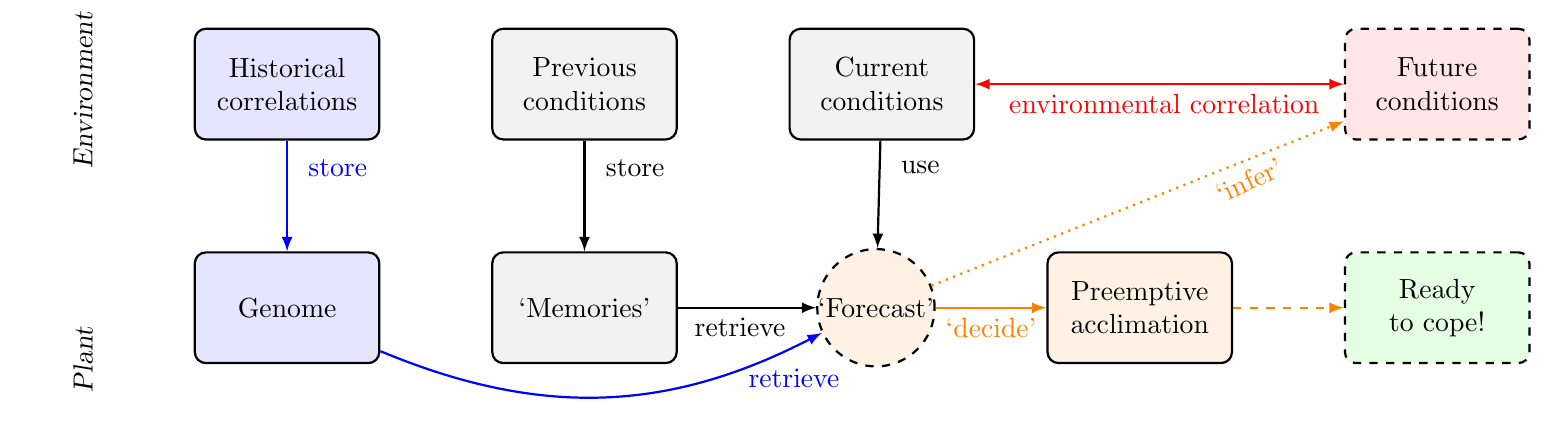
\begin{tikzpicture}[auto]
    \node [a, rotate=90] (environment) {\textsl{Environment}};
    \node [b, right = of environment, fill=blue!10] (history) {Historical correlations};
    \node [b, right = of history] (stress) {Previous conditions};
    \node [b, right = of stress] (data) {Current conditions};\pause
    \node [b, below = of stress] (memory) {`Memories'};
    \node [c, right = of memory] (info) {`Forecast'};
    \node [b, below = of history, fill=blue!10] (genome) {Genome};
    \node [a, rotate=90, left = of genome] (plant) {\textsl{Plant}};\pause
    \node [b, right = of info, fill=orange!10] (acclimation) {Preemptive acclimation};
    \node [d, right = of acclimation, fill=green!10] (ready) {Ready to cope!};
    \node [d, above = of ready] (stress2) {Future conditions};\pause

    \path [l] (stress) -- (memory) node[near start,right]{\hspace{0.4em}store};
    \path [lb] (history) -- (genome) node[near start, right]{\hspace{0.4em}store};\pause
    \path [l] (data) -- (info) node[near start,right]{\hspace{0.4em}use};
    \path [l] (memory) -- (info) node[near start,below]{\hspace{2em}retrieve};
    \path [lb] (genome) edge [bend right=25]  node[near end, right]{\hspace{1em}retrieve} (info);\pause
    \path [lr] (stress2) -- (data) node[near end,below]{\hspace{7em}environmental correlation};\pause
    \path [lo, dotted] (info) -- (stress2) node[near end,below,rotate=25]{`infer'};\pause
    \path [lo] (info) -- (acclimation) node[near start,below]{\hspace{2em}`decide'};\pause
\path [lo, dashed] (acclimation) -- (ready); 

\end{tikzpicture}
\end{frame}

\begin{frame}
\begin{figure}[h]
\sffamily
\centering
\tiny
  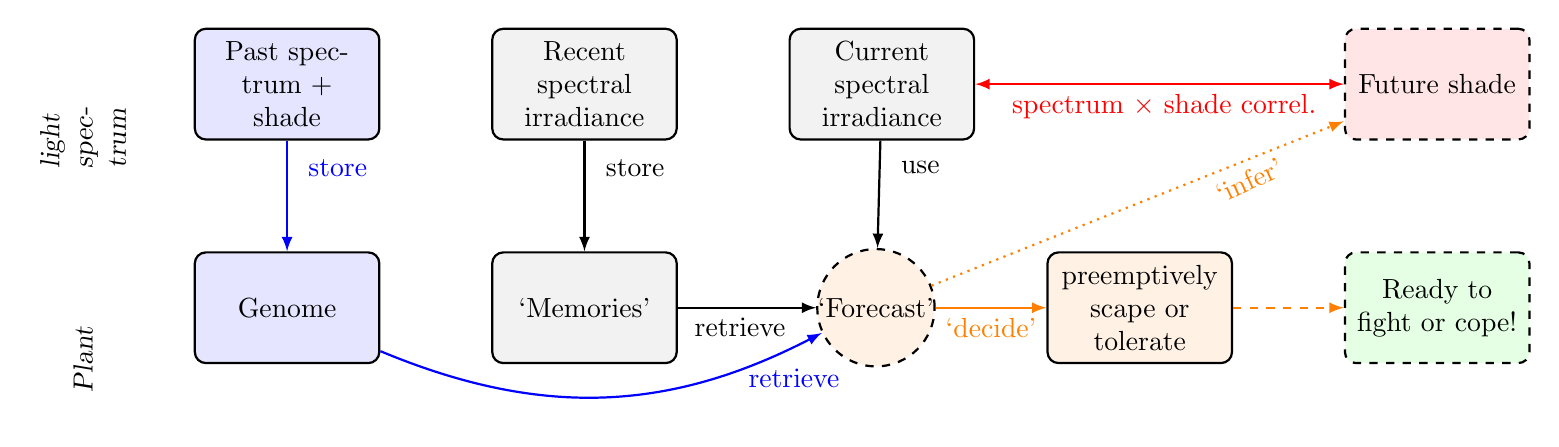
\begin{tikzpicture}[auto]
    \node [a, rotate=90] (environment) {\textsl{light spectrum}};
    \node [b, right = of environment, fill=blue!10] (history) {Past spectrum + shade};
    \node [b, below = of history, fill=blue!10] (genome) {Genome};
    \node [a, rotate=90, left = of genome] (plant) {\textsl{Plant}};
    \node [b, right = of history] (stress) {Recent\\ spectral irradiance};
    \node [b, right = of stress] (data) {Current spectral irradiance};
    \node [b, below = of stress] (memory) {`Memories'};
    \node [c, right = of memory] (info) {`Forecast'};
    \node [b, right = of info, fill=orange!10] (acclimation) {preemptively scape or tolerate};
    \node [d, right = of acclimation, fill=green!10] (ready) {Ready to fight or cope!};
    \node [d, above = of ready] (stress2) {Future shade};

    \path [l] (data) -- (info) node[near start,right]{\hspace{0.4em}use};
    \path [l] (memory) -- (info) node[near start,below]{\hspace{2em}retrieve};
    \path [l] (stress) -- (memory) node[near start,right]{\hspace{0.4em}store};
    \path [lb] (history) -- (genome) node[near start, right]{\hspace{0.4em}store};
    \path [lb] (genome) edge [bend right=25]  node[near end, right]{\hspace{1em}retrieve} (info);
    \path [lo] (info) -- (acclimation) node[near start,below]{\hspace{2em}`decide'};
     \path [lo, dotted] (info) -- (stress2) node[near end,below,rotate=25]{`infer'};
   \path [lr] (stress2) -- (data) node[near end,below]{\hspace{7em}spectrum $\times$ shade correl.};
    \path [lo, dashed] (acclimation) -- (ready) node[near start,below]{};

\end{tikzpicture}
%%\vspace{-6ex}
%\caption{\footnotesize\sffamily Information use in preemptive acclimation to drought by perception of UV-B radiation. Arrows represent flows of information: \textcolor{blue}{\textbf{blue}} = retrieved from genome (stored during earlier generations), \textbf{black} = acquired and/or `memorized' during an individual's lifetime, \textcolor{red}{\textbf{red}} = lagged correlation between UV-B radiation and drought (e.g.\ low soil water content and high evaporative demand), \textcolor{orange}{\textbf{orange}} = represents the outcome of `data processing'. The outcome is a `decision' on how to adjust function, morphology and development to achieve drought tolerance based on an `implicit forecast of impending drought'. Time runs from left to right, with dashed boxes representing the future. `Conditions' refer to both external environment and plant's internal status.}\label{fig:drought:info}
\end{figure}
\end{frame}

\section{Organism-independent definitions}

\begin{frame}[<+->]
  \frametitle{Learning}
  \begin{itemize}
    \item In some recent plant science papers \emph{habituation} is equated to \emph{learning}
    \item To me this is not real learning\ldots
    \item I would define \emph{deep learning} to be able to use as sources of information correlations that were not experienced
    or used as sources of information by ancestors\ldots
    \item (assuming that plants cannot learn from each other\ldots)
  \end{itemize}
\end{frame}

\begin{frame}[<+->]
  \frametitle{Itelligence}
  \begin{itemize}
    \item Could we derive from \emph{systems intelligence} a definition of intelligence
    that is independent of the physiological `implementation' in different organisms?
  \end{itemize}
\end{frame}

\begin{frame}[<+->]
  \frametitle{Behaviour}
  \begin{itemize}
    \item I do not have problems with \emph{plant behaviour}, I think it is just a
    question of the speed at which the behaviour takes place, and the low visibility
    by the smaller distances for movement.
  \end{itemize}
\end{frame}

\begin{frame}[<+->]
  \frametitle{How does the problem look?}
  \begin{itemize}
    \item from philosophy?
    \item evolution?
    \item from animal behaviour?
    \item animal sensory ecology?
    \item \ldots
  \end{itemize}
\end{frame}
\section{References}

\begin{frame}[<+->]
\frametitle{Thanks for listening!}
\begin{center}
%\includegraphics[height=0.8\textheight]{figures/sky_and_trees.jpg}
\end{center}
\end{frame}

\begin{frame}[<+->]
\frametitle{Contact and acknowledgements}
For additional information on our research, please have a look at our web site at \url{http://blogs.helsinki.fi/senpep-blog/}.\\[2ex]

I can be contacted at \url{mailto:pedro.aphalo@helsinki.fi}\\[2ex]

We acknowledge the support of the Academy of Finland (decision 252548).

\begin{center}

\end{center}
\end{frame}


\end{document}
